% This tells the program how to initially format my document.
\documentclass[dvipsnames]{article}

% List of packages to be included for the use of special commands and symbols.
\usepackage{amsmath,amssymb,amsthm}
\usepackage{mathtools}
\usepackage{mathrsfs}
\usepackage[letterpaper,margin=1in]{geometry}
\usepackage{enumitem}
%% remove ligatures (e.g. ``ff") to allow text copying from PDF
\usepackage{microtype}
\DisableLigatures{encoding = *, family = * }
\usepackage{fancyhdr}
\usepackage[T1]{fontenc}
\usepackage{lmodern}
\usepackage[USenglish]{babel}

\usepackage{tikz}
\usepackage{float}
\usepackage{listings}
\usepackage{xcolor}
\usepackage{multicol}

\definecolor{lispgreen}{RGB}{154, 228, 151}
\definecolor{lightgray}{gray}{0.97}
\definecolor{violet}{rgb}{0.8, 0, 0.7}

\lstdefinestyle{cpp}{
    language=C++,
	basicstyle=\fontsize{9}{11}\ttfamily,
	keywordstyle=\color{blue}\ttfamily,
	stringstyle=\color{red}\ttfamily,
	commentstyle=\color{OliveGreen}\ttfamily,
	morecomment=[l][\color{magenta}]{\#},
	tabsize=2,
    showstringspaces=false,
    backgroundcolor=\color{lightgray},
    numbers=left,
    stepnumber=5,
    numberstyle=\tiny
}
\lstdefinestyle{out}{
    basicstyle=\fontsize{9}{11}\ttfamily,
    tabsize=4,
    backgroundcolor=\color{lightgray},
    morecomment=[l][\color{OliveGreen}]{\#},
    numbers=none
}

\setlength{\parindent}{0cm}

\pagestyle{fancy}
\rhead{\large Alexander Novotny}
\lhead{\large CS 485 PA1}
\setlength{\headheight}{14pt}

\title{CS 485 Programming Assignment 1}
\date{March 4, 2019}
\author{Alexander Novotny}

\begin{document}
\pagenumbering{roman}

\maketitle

\section*{Problem 1}
\subsection*{Approach}
As discussed in the assignment, we wish to solve a set of equations defined by an affine transformation:
\begin{align*}
	\hat{P}_1 &= AP_1 + b,\\
	\hat{P}_2 &= AP_2 + b,\\
	\hat{P}_3 &= AP_3 + b,\\
	\hat{P}_4 &= AP_4 + b,\\
\end{align*}
where $(P_1, P_2, P_3, P_4)$ are the original eye, nose, and mouth locations (found by hand) and $(\hat{P}_1, \hat{P}_2, \hat{P}_3, \hat{P}_4)$ are their fixed goal locations in the normalised images. This system can be reduced to an equivalent system
\begin{align*}
	\hat{p}_x &= Pc_1,\\
	\hat{p}_y &= Pc_2,\\
\end{align*}
where
\begin{align*}
	\hat{p}_x &= \begin{bmatrix}\hat{X}_1\\\hat{X}_2\\\hat{X}_3\\\hat{X}_4\end{bmatrix}, &
	\hat{p}_y &= \begin{bmatrix}\hat{Y}_1\\\hat{Y}_2\\\hat{Y}_3\\\hat{Y}_4\end{bmatrix}, &
	c_1 &= \begin{bmatrix}a_{11}\\a_{12}\\b_1\end{bmatrix}, &
	c_2 &= \begin{bmatrix}a_{21}\\a_{22}\\b_2\end{bmatrix},
\end{align*}
and
\[
	P =
	\begin{bmatrix}
		X_1 & Y_1 & 1\\
		X_2 & Y_2 & 1\\
		X_3 & Y_3 & 1\\
		X_4 & Y_4 & 1
	\end{bmatrix}.
\]

Unfortunately, since this an overdetermined system, an exact solution is unlikely to exist. So we find the closest (least squares) solution using Singular Value Decomposition (SVD) and back-substitution. This lets us construct $\tilde{A}$ and $\tilde{b}$ from our least squares solutions $\tilde{c}_1, \tilde{c}_2$ and acquire a close enough affine transformation
\[
	\hat{P} \approx \tilde{A}P + \tilde{b},
\]
for all of our fixed points.

% \begin{figure}
% 	\begin{tikzpicture}
% 		\node[anchor=south west,inner sep=0] (image) at (0,0) {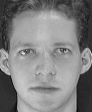
\includegraphics[width=.1\textwidth]{Sample1-1.png}};
% 		\begin{scope}[x={(image.south east)},y={(image.north west)}]
% 			\draw[red,ultra thick,rounded corners] (0.62,0.65) rectangle (0.78,0.75);
% 		\end{scope}
% 	\end{tikzpicture}
% \end{figure}

Unfortunately, this transformation goes from our original image to our normalised image, which is smaller, so multiple pixels in the original images might map to the same pixel in our normalised image. To fix this, we instead examine the transformation
\[
	P \approx \tilde{A}^{-1}(\hat{P} - \tilde{b}),
\]
which allows us to go from pixels in our normalised image to pixels in our original image.

\newpage

\subsection*{Recovered parameters}
\lstset{style=out}
\lstinputlisting[float=h!, multicols=3,caption={Recovered affine transformation parameters},label={out:parameters}]{parameters.out}

\newpage

\subsection*{Normalised images}
\begin{multicols}{3}
\begin{figure}[H]
	\centering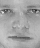
\includegraphics{Out-JPG/S1/1.jpg}
	\caption{S1/1.pgm}
\end{figure}
\begin{figure}[H]
	\centering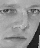
\includegraphics{Out-JPG/S1/2.jpg}
	\caption{S1/2.pgm}
\end{figure}

\begin{figure}[H]
	\centering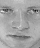
\includegraphics{Out-JPG/S1/3.jpg}
	\caption{S1/3.pgm}
\end{figure}

\begin{figure}[H]
	\centering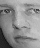
\includegraphics{Out-JPG/S1/4.jpg}
	\caption{S1/4.pgm}
\end{figure}

\begin{figure}[H]
	\centering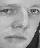
\includegraphics{Out-JPG/S1/5.jpg}
	\caption{S1/5.pgm}
\end{figure}

\begin{figure}[H]
	\centering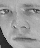
\includegraphics{Out-JPG/S1/6.jpg}
	\caption{S1/6.pgm}
\end{figure}

\begin{figure}[H]
	\centering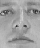
\includegraphics{Out-JPG/S1/7.jpg}
	\caption{S1/7.pgm}
\end{figure}

\begin{figure}[H]
	\centering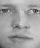
\includegraphics{Out-JPG/S1/8.jpg}
	\caption{S1/8.pgm}
\end{figure}

\begin{figure}[H]
	\centering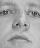
\includegraphics{Out-JPG/S1/9.jpg}
	\caption{S1/9.pgm}
\end{figure}

\begin{figure}[H]
	\centering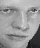
\includegraphics{Out-JPG/S1/10.jpg}
	\caption{S1/10.pgm}
\end{figure}

\begin{figure}[H]
	\centering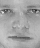
\includegraphics{Out-JPG/S1/1.jpg}
	\caption{S2/1.pgm}
\end{figure}
\begin{figure}[H]
	\centering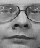
\includegraphics{Out-JPG/S2/2.jpg}
	\caption{S2/2.pgm}
\end{figure}

\begin{figure}[H]
	\centering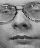
\includegraphics{Out-JPG/S2/3.jpg}
	\caption{S2/3.pgm}
\end{figure}

\begin{figure}[H]
	\centering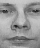
\includegraphics{Out-JPG/S2/4.jpg}
	\caption{S2/4.pgm}
\end{figure}

\begin{figure}[H]
	\centering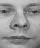
\includegraphics{Out-JPG/S2/5.jpg}
	\caption{S2/5.pgm}
\end{figure}

\begin{figure}[H]
	\centering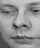
\includegraphics{Out-JPG/S2/6.jpg}
	\caption{S2/6.pgm}
\end{figure}

\begin{figure}[H]
	\centering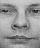
\includegraphics{Out-JPG/S2/7.jpg}
	\caption{S2/7.pgm}
\end{figure}

\begin{figure}[H]
	\centering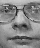
\includegraphics{Out-JPG/S2/8.jpg}
	\caption{S2/8.pgm}
\end{figure}

\begin{figure}[H]
	\centering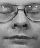
\includegraphics{Out-JPG/S2/9.jpg}
	\caption{S2/9.pgm}
\end{figure}

\begin{figure}[H]
	\centering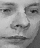
\includegraphics{Out-JPG/S2/10.jpg}
	\caption{S2/10.pgm}
\end{figure}

\vfill\null
\end{multicols}

\subsection*{Results}
As seen in the next section, the transformation does an exceedingly good job at transforming the facial features to be exactly where I want them to be. The average error is always much less than 1.

\subsection*{Average error}
\lstset{style=out}
\lstinputlisting[float=h!, multicols=2,caption={Average transformation error for fixed facial features},label={out:error}]{error.out}


\end{document}